\chapter{Clustering}


\section{Common Setting}

The data preparation common to all different clustering algorithms consists of three main steps: categorical attributes dropping, outlier removal and scaling.
The removal of outliers has been performed by applying the IQR method, i.e. cutting all the points that have at least one attribute whose value falls out of the IQR of the column; the threshold value used for the computation of the IQR is the default one of 1.5.\\
Than the remaining points have been scaled with the Min-Max scaling method for two main reasons:
\begin{itemize}
    \item Empirically, it leads to better clustering results with respect to the Standard scaling method, maybe due to skewed (asymmetric) or not approximately Gaussian distributions of some defined indicators and to features with very different scales and variances (the impact of features with large variances may still be noticeable, especially if the distribution is not close to Gaussian). Using the min-max scaling method guarantees that all the attribute values fall into the same range ([0, 1]) ensuring a consistent scale across features.
    \item The fact that the scaled values are in a specific range ([0, 1]) makes them easily interpretable.
\end{itemize}
All the explored clustering approaches, respectively K-means, density-based (DBSCAN) and hierarchical have been applied to different data spaces:
\begin{itemize}
    \item the data space defined only by the original attributes (without the defined indicators),
    \item the data space defined by both original attributes and indicators,
    \item the data space defined by only the defined indicators (without the original attributes),
    \item the data space obtained applying dimensionality reduction (attributes cutting based on variance and correlation) to each of the preceding spaces.
\end{itemize}
In the experiments involving indicators, the outlier removal has been performed before the augmentation with the indicators (i.e. only on the original features), in order to compare the performances on the same set of points represented on a different space.\\
The difference in results between the original data space and the augmented data space measures the impact of the defined indicators on the clustering, while the difference in results between the indicators data space and the data space containing original attributes measures how much of the useful original information the indicators contain/preserve.\\
The dimensionality reduction based on variance and correlation consists in two steps:
\begin{enumerate}
    \item cut all the features that have a very low variance in the entire dataset;
    \item cut all the features that have a very low variance in the entire dataset;
\end{enumerate}
The reduction is applied on the scaled data, using a variance threshold of 0.01 and a correlation threshold of 0.25.\\
Each clustering scenario is evaluated by comparing the resulting silhouette score with the silhouette score of the same clustering algorithm applied on a randomly generated dataset in the same data space.\\
A random dataset containing the same number of points of the true dataset without outliers is generated in the original feature space, respecting the value range and the type of each attribute. Then the augmented dataset and the indicators dataset are computed from this random data.\\
The clustering algorithms have been performed using euclidean distance as a metric.\\
Finally an interpretation of the resulting clusters is given looking at the distribution of each attribute (including categorical ones) inside the clusters.

\section{K-means}

Note: The same clustering procedure is applied to each data space.

\subsection{K Selection and Evaluation}

One of the choices to perform for applying K-means clustering is the choice of the number of clusters k. In the experiments the tried values are the ones in the interval [2, 20]. For each k a K-means clustering is performed and a silhouette score is computed; while the clustering is performed on the entire set of points, the silhouette score is computed for samples of points, since it requires too much time. After a first computation of the score, the best k value (the one with the highest score) and the near values are selected, assuming a sort of locality property, and another silhouette score computation is performed on them, increasing the sample sizes.\\
Finally only the best k is selected and a final silhouette score computation is performed on it, further increasing the sample sizes, in such a way to have a more accurate estimate of the silhouette on the whole set of points.\\
In Table xx are reported the number of samples and sample sizes of each silhouette score computation.\\
%Table

\subsection{Results}

In Fig xx and Table xx are summarized the clustering results.\\
%figures and tables
The clustering applied to the data spaces reduced using variance and correlation informations gives better result both in terms of absolute silhouette score and in terms of score difference from the random case.\\
Moreover the reduced scenarios show lower variances in the silhouette score computations than the full data space score comutations.

\subsection{Analysis}

\subsubsection{Centroids}

Looking at the centroids, one can observe that attributes regarding males and injured participants are distinguishing aspects that differ the centroids of the most of the clusterings performed. These aspects can be observed also looking at the males and injured attributes distributions in the clusters.
%figs of centroids and distributions

\subsubsection{Categorical Attributes Distributions Among the Clusters}

For the analysis of categorical distributions among clusters, we consider the clusterings on the reduced data, which have better results both in terms of score and in terms of difference with the random case.



\begin{figure}[ht]
    \centering
    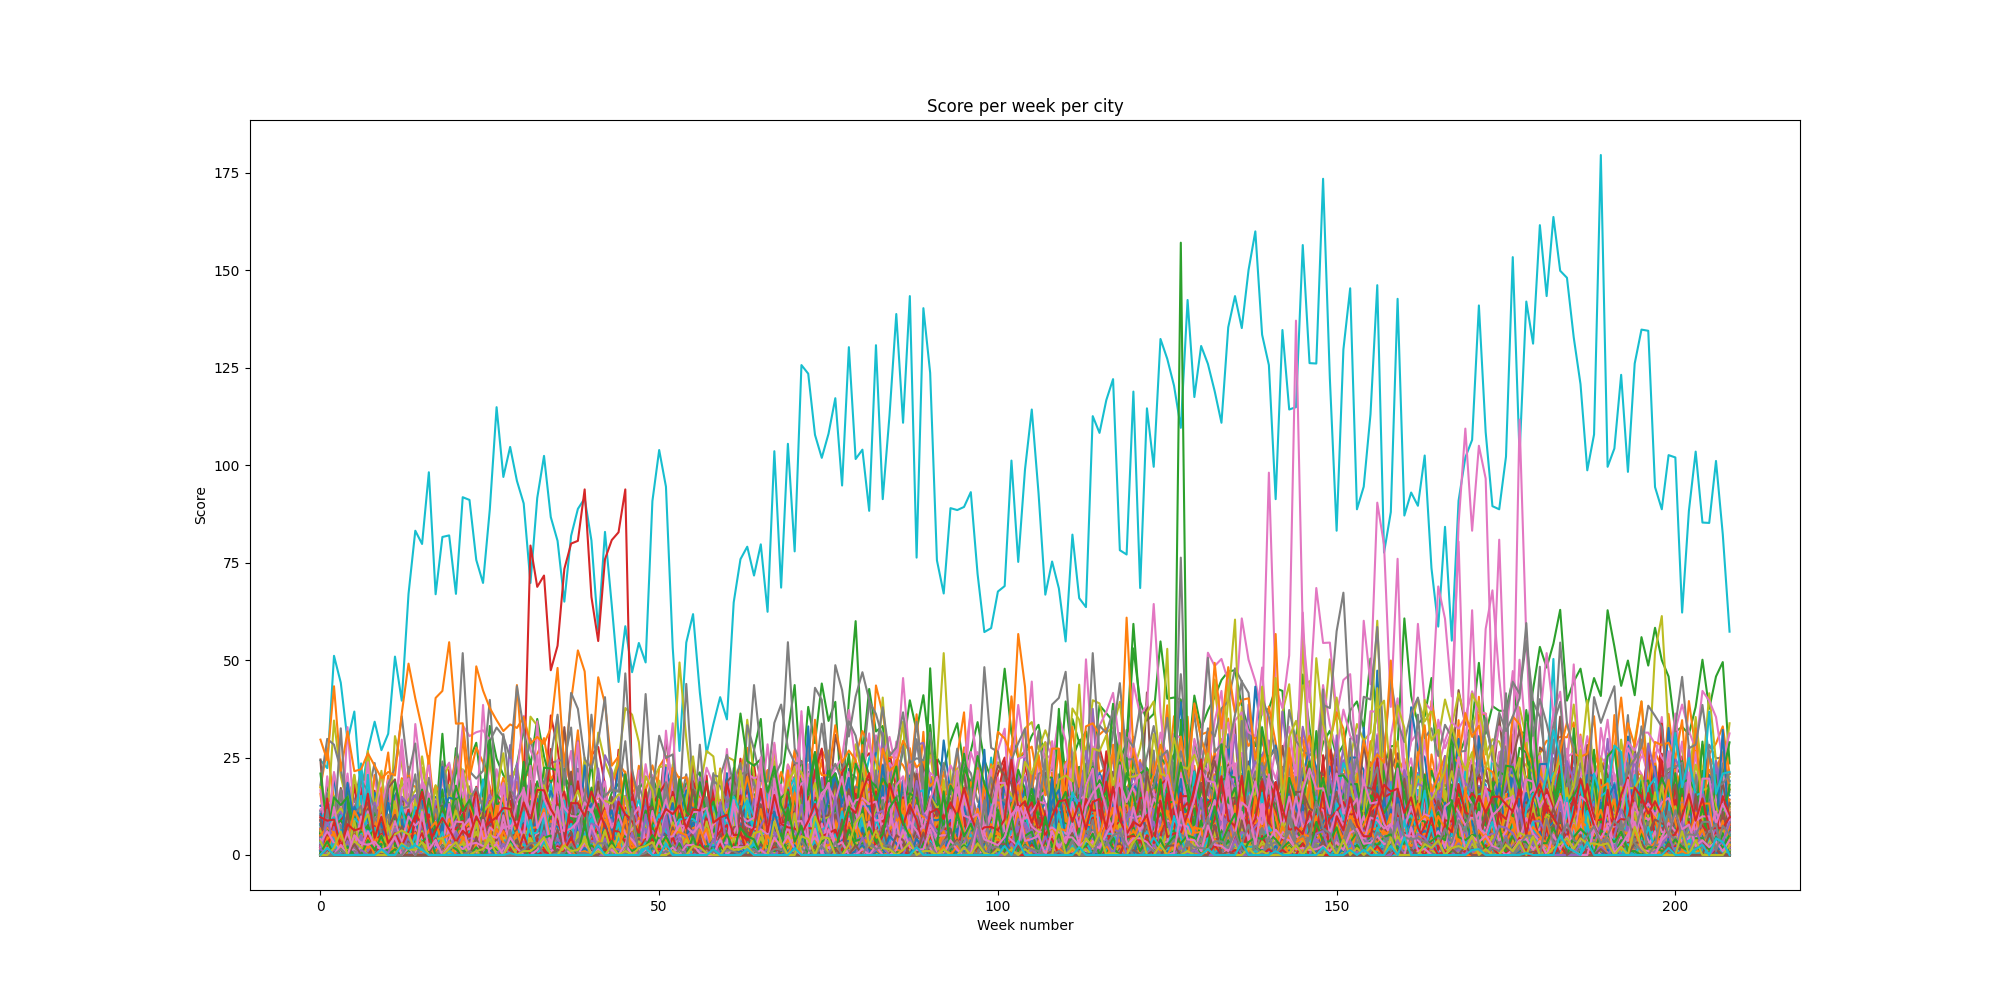
\includegraphics[width= 0.8\textwidth]{images/Capitolo1/score_per_week_per_city.png} 
    \caption{Questa è un'immagine} 
    \label{fig:score_per_week_per_city}
\end{figure}

\subsection{Scaled Timeseries}

We decided to also test the clustering on the timeseries scaled with the standard scaler and the minmax scaler, to see if doing so would result in better clusters

In the following figure we can see the plot for all the timeseries scaled in this way

\begin{figure}[ht]
    \centering
    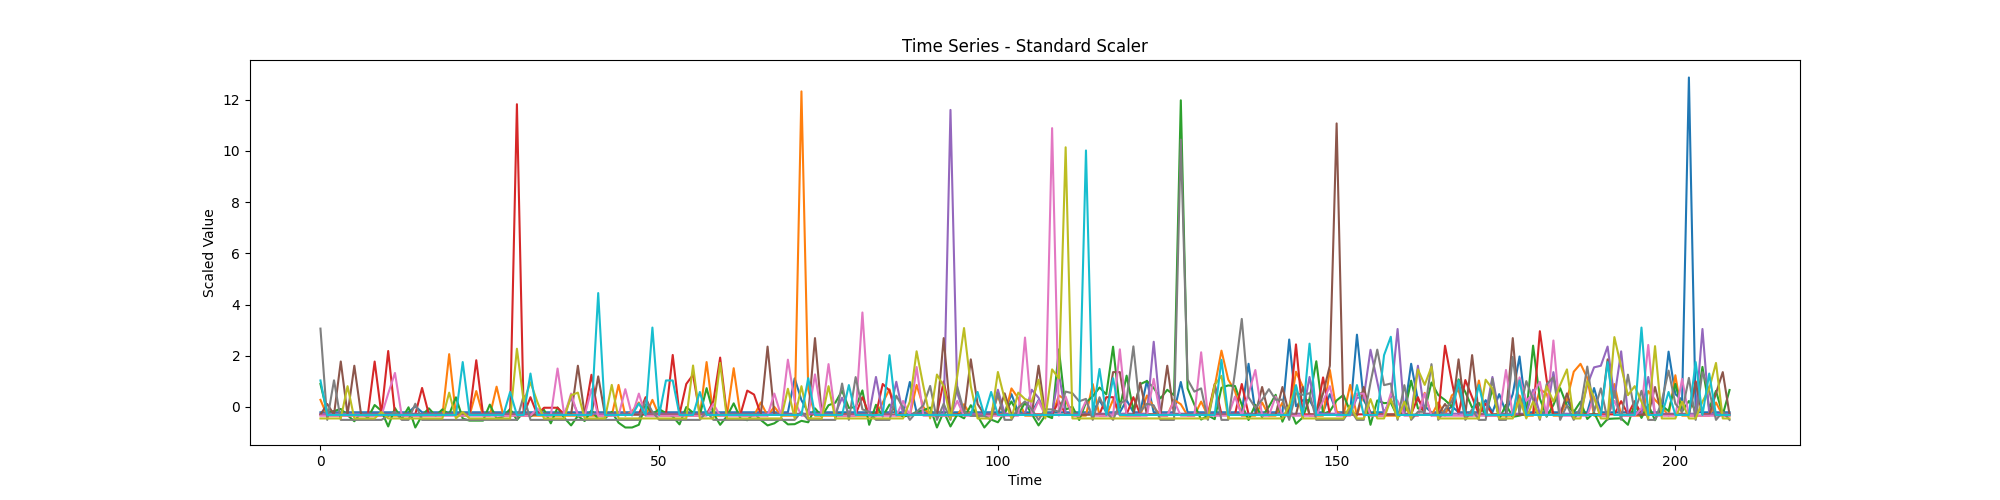
\includegraphics[width= 0.8\textwidth]{images/Capitolo1/time_series_standard_scaler.png} 
    \caption{Questa è un'immagine} 
    \label{fig:time_series_standard_scaler}
\end{figure}

\begin{figure}[ht]
    \centering
    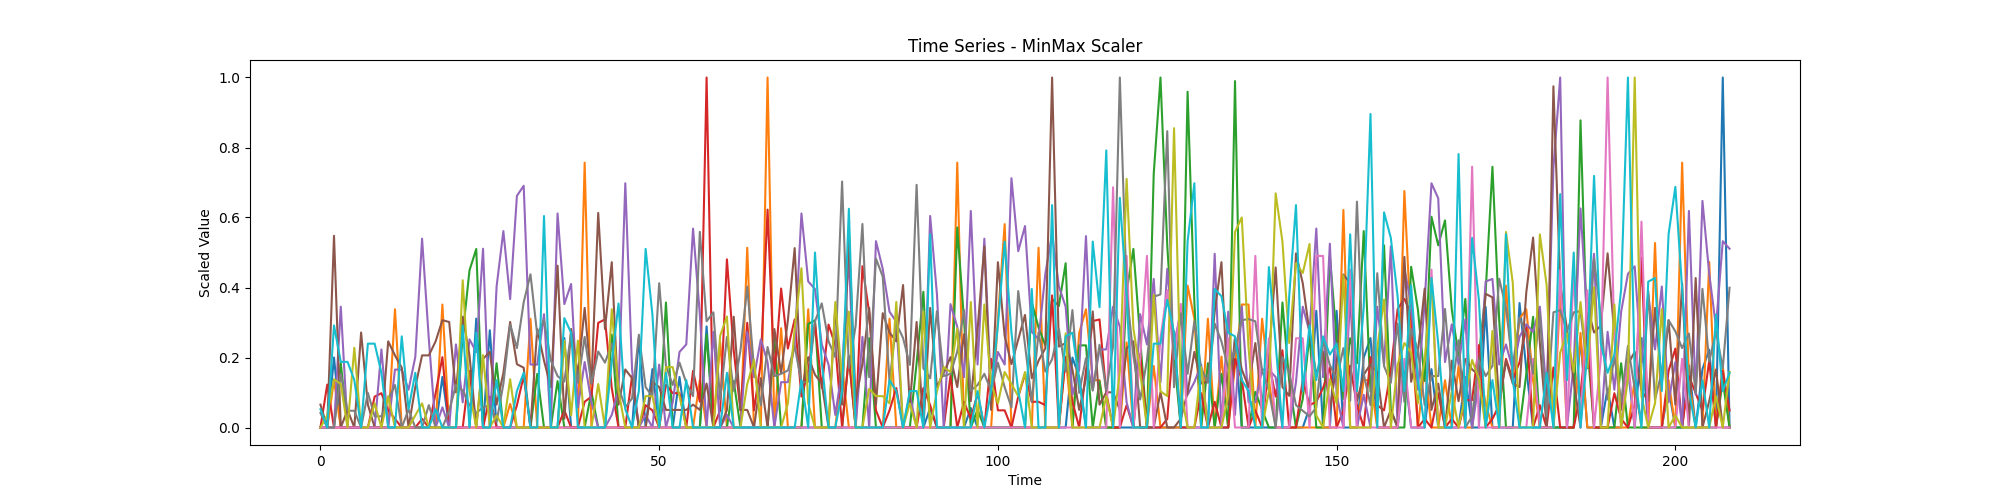
\includegraphics[width= 0.8\textwidth]{images/Capitolo1/time_series_minmax_scaler.png} 
    \caption{Questa è un'immagine} 
    \label{fig:time_series_minmax_scaler}
\end{figure}


\section{Clustering}

For the cluster analysis we decided to not test most of the algorithms because we already tested them in previous section of the project.
So we decided to concentrate on K-means on the raw time series and on their features.
We also skipped the euclidean distance and decided to use the Dynamic Time Warping (DTW) mainly because it is better suited to capture time series with varying pattern, time shifts or speed, all things that euclidean distance could miss.


\subsection{Clustering on the raw Timeseries}

We applied K-means on the original timeseries and also on the one scaled with the standard scaler and the minmax scaler.

To find the best number of cluster we used the same technique that we used in the clustering of the incident dataset, the silhouette score.

As seen in the table, both the standard scaler and the minmax scaler resulted in a significant reduction of the clustering score, while the original timeseries reached a 0.8. 


\subsection{Clustering on the feature of the Timeseries}

Another technique often used when dealing with Timeseries is to reduce each one of them to a vector containing some significant feature of the Timesearies, such as mean, variance, kurtosis ecc..  and then apply the clustering algorithms to those points.

Same as the clustering on raw time series we performed K-means on the initial timeseries, the timeseries scaled with the standard scaler and the one scaled with the minmax scaler.
We registered a significant increase in the silhouette score for all three of the timeseries, a number much greater than the one for the corresponding initial timeseries.
In particular feature clustering on the original timeseries seems to best differentiate the two clusters found





\subsection{Comparison of the clustering with a random walk}

To test how well K-means worked on our timeseries we generated the same number of random walk with the same number of points and with the same min and max value as our standard timeseries.

We then procedeed to use K-means on the standard random timeseries and discovered a silhouette score close to zero, confirming that our time series were clustered better than randomly.
The same conclusion was reached also on the feature based cluster, in which even though the clustering on the random timeseries reached $0.50$ it was still significantly lower than the corresponding score on the original timeseries




\section{Motif and Anomaly Detection}

The timeseries chosen for the motif discovery are the two cluster centroids found with K-means in the previous point.
Altough the significance of those two timeseries could be discussed, the idea behind it is that no timeseries is significant enough to conduct this kind of analysis on.
We should consider them equal and in this way analyze each city one by one.
Because it was not possible to study that many city, we opted to take the two timeseries that describe the two different clusters.
Another possible analysis could be conducted on a small sample from each of those clusters, but still this analysis is not that much more significant.

The only interesting thing that we can notice is the 'absence' of motifs in the random series, which is to be expected, while we can always find some motif in our timeseries, scaled or not scaled.

As far as Anomaly detection, we conducted it on the non scaled Timeseries, and we were able to find a couple of anomalies, but also these anomalies cannot really be interpreted in a nice way.

For comparison, we also took a couple of the cities with the highest score and the one with the lowest and conducte the motif and anomaly discovery on those.

The results were similar to the one on the cluster centers, because nothing particularly interesting emerged, except that the motif alternated between each other.



\section{Shapelets}

For the analysis on the Shapelets of the time series, we needed to create  new indicator.
The new score for each city is defined as follows:
\textit{Score\textunderscore Shapelet $=$ number of incidents in that week + number of participants in incidents in that week}

In this case the main idea behind this score is that by summing the number of incidents and the number of people involved we could get a decent indirect correlation with the given label is\textunderscore killed.

We chose the threshold after which a timeseries would be considered as a positive is\textunderscore killed value, in a way to make the number of positive city almost the same as the negative cities, mainly to make classification more precise.

For the shapelet extraction, due to the high computational cost of the algorithms, decided to take only a small sample of the time series and extract the shapelet from those.
We also tried to use the tensorflow library but gave results that suggested some kind of problem, so we used the alternative method for finding the shapelets (pyts library)

Despite the low number of samples, the F1 score of the classifier got an accuracy of 0.83 and a decent ROC curve




















